% !TEX TS-program = xelatex
% !TEX encoding = UTF-8 Unicode

% Tennessee Technological University
% ME4020 - Fall 2022
% Tristan Hill - November 09, 2022
% Power Screws - This lecture is based on Section 15.2 Power Screws, Machine Design by Norton 6th ed.

\documentclass[fleqn]{beamer} % for presentation (has nav buttons at bottom)

% custom preamble
%\usepackage{/home/tntech.edu/thill/courses/machine_design/machine_design_lecture}
\usepackage{/home/thill/courses/machine_design/machine_design_lecture}


\newcommand{\MNUM}{1\hspace{2mm}} % Module number
\newcommand{\TNUM}{1\hspace{2mm}} % Topic number 
\newcommand{\moduletitle}{Power Screws and Bolted Connections} 
\newcommand{\lecturetitle}{Power Screws} 

\newcommand{\sectiontitleI}{Overview and Applications}
\newcommand{\sectiontitleII}{Threads for Power Transmission}
\newcommand{\sectiontitleIII}{Force and Torque Analysis}
\newcommand{\sectiontitleIV}{Friction and Efficiency}
\newcommand{\sectiontitleV}{ Design Considerations}

\author{ME4020 - Applied Machine Design}
\title{\GD \moduletitle}
\date{Mechanical Engineering\vspc Tennessee Technological University}

\begin{document}

\lstset{language=MATLAB,basicstyle=\ttfamily\small,showstringspaces=false}

\frame{\titlepage \center\begin{framed}\Large \textbf{\lecturetitle}\end{framed} \vspace{5mm}}

% Section 0 - Outline
\frame{
	
	\large \textbf{\lecturetitle} \vspace{3mm}\\
	
	\begin{itemize}
	
		\item \hyperlink{sectionI}{\color{black}\sectiontitleI}	\vspace{3mm} % Section I
		\item \hyperlink{sectionII}{\color{black}\sectiontitleII}	\vspace{3mm} % Section II
		\item \hyperlink{sectionIII}{\color{black}\sectiontitleIII}	\vspace{3mm} %Section III
		\item \hyperlink{sectionIV}{\color{black}\sectiontitleIV}	\vspace{3mm} %Section IV
		\item \hyperlink{sectionV}{\color{black}\sectiontitleV} %Section IV	
	
	\end{itemize}

}

% Section I
\section{\sectiontitleI}

	% Section I - Frame I
	\begin{frame}[label=sectionI] \small
		\frametitle{\sectiontitleI}	

		\begin{multicols}{2}
			A power screw is a machine component that converts rotational motion into linear motion. This is neccesary in variety of applications. 

			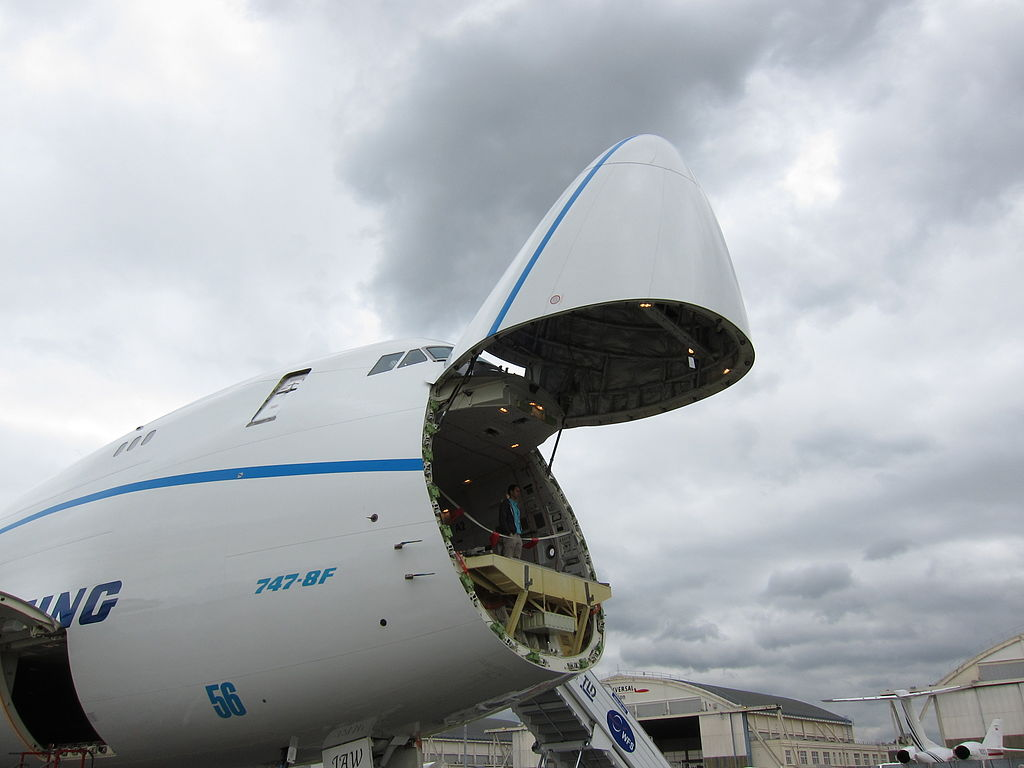
\includegraphics[scale=0.135]{images/1024px-Nose_cargo_door_of_Boeing_747-8F.jpg}

			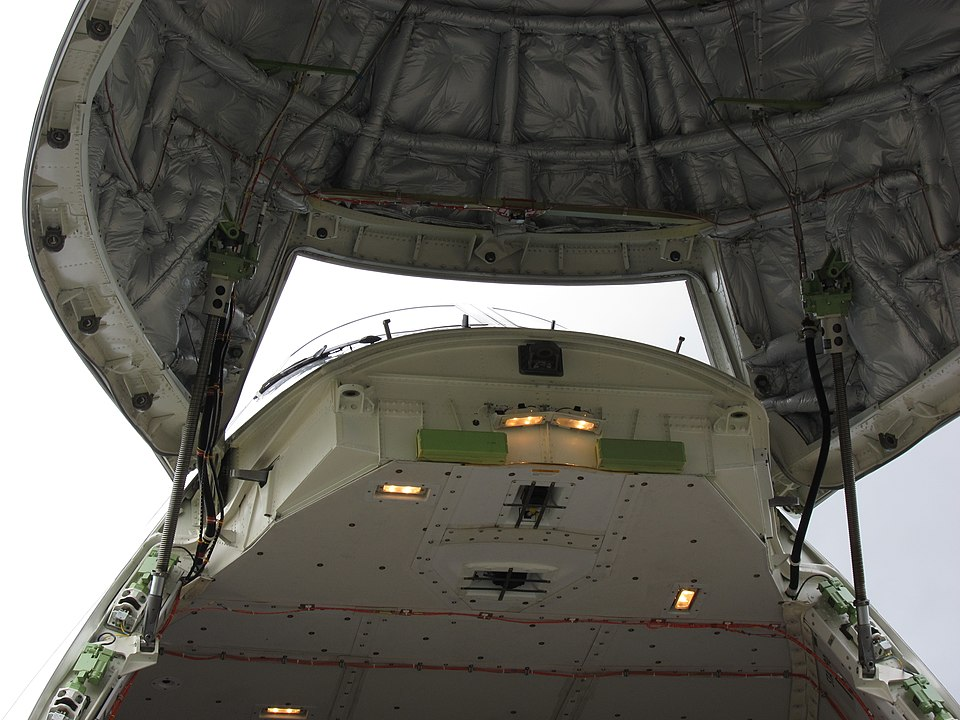
\includegraphics[scale=.175]{images/960px-Detail_of_raised_nose_cargo_door_of_Boeing_747-8F.jpeg}
			\tiny{Leadscrews are used to raise and lower the front door of the Boeing 747-8F Freighter aircraft}
		\end{multicols}

		{\tiny images: \href{https://en.m.wikipedia.org/wiki/File:Nose_cargo_door_of_Boeing_747-8F.jpg}{wikimedia}, \href{https://en.wikipedia.org/wiki/Leadscrew}{wikipedia} }

	\end{frame}


	% Section I - Frame II
	\begin{frame}[label=sectionI] \small
		\frametitle{\sectiontitleI}	
		
		\begin{multicols}{2}
		Common Applications:
		\begin{itemize}
			\item automotive jack and jack post
			\item machining tool positioning
			\item automatic doors and gates 
			\item aircraft control surfaces
			\item automation/production machines	
		\end{itemize}

		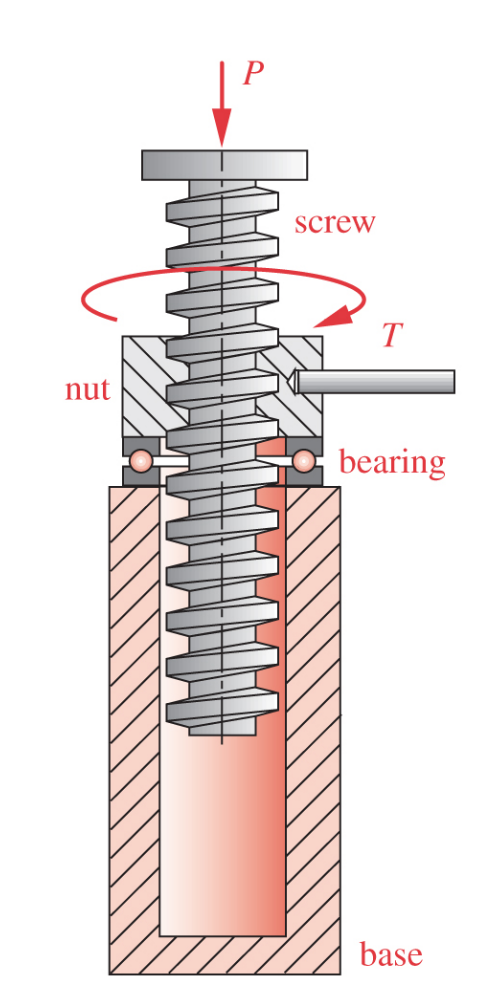
\includegraphics[scale=0.1]{images/figure_15_4.png}
		

		\end{multicols}

	\end{frame}

	% Section I - Frame II
	\begin{frame}[label=sectionI] \small
		\frametitle{\sectiontitleI}	
		Machining Tool Positioning - 3 Axis Mill

		\begin{multicols}{2}
			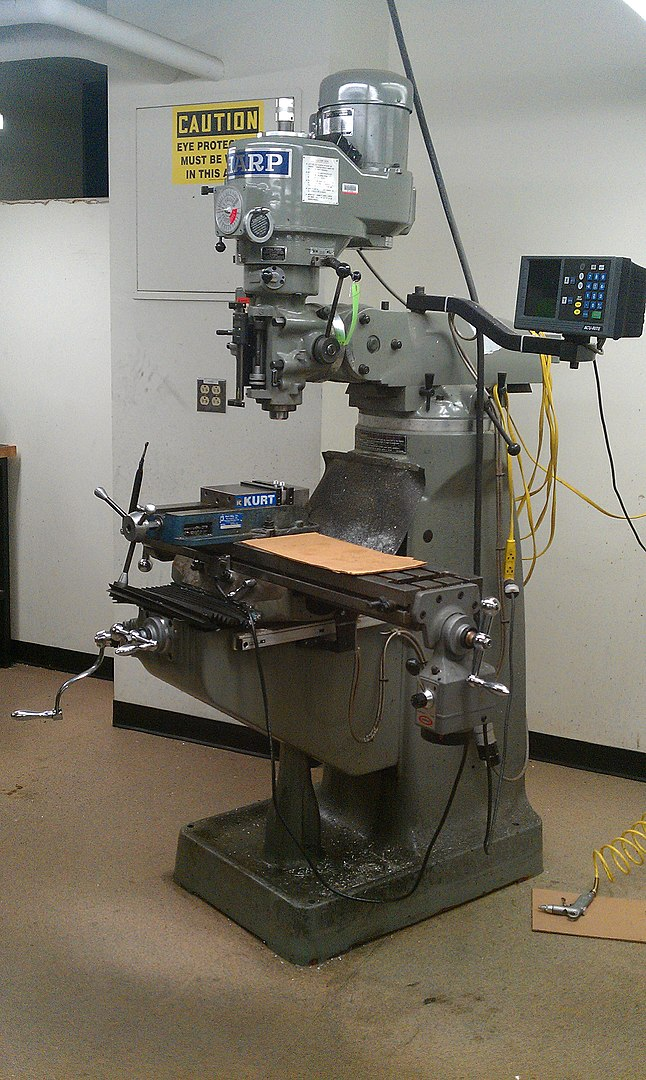
\includegraphics[scale=0.15]{images/Sharp_3_Axis_Vertical_Mill_Full_View.jpeg}

			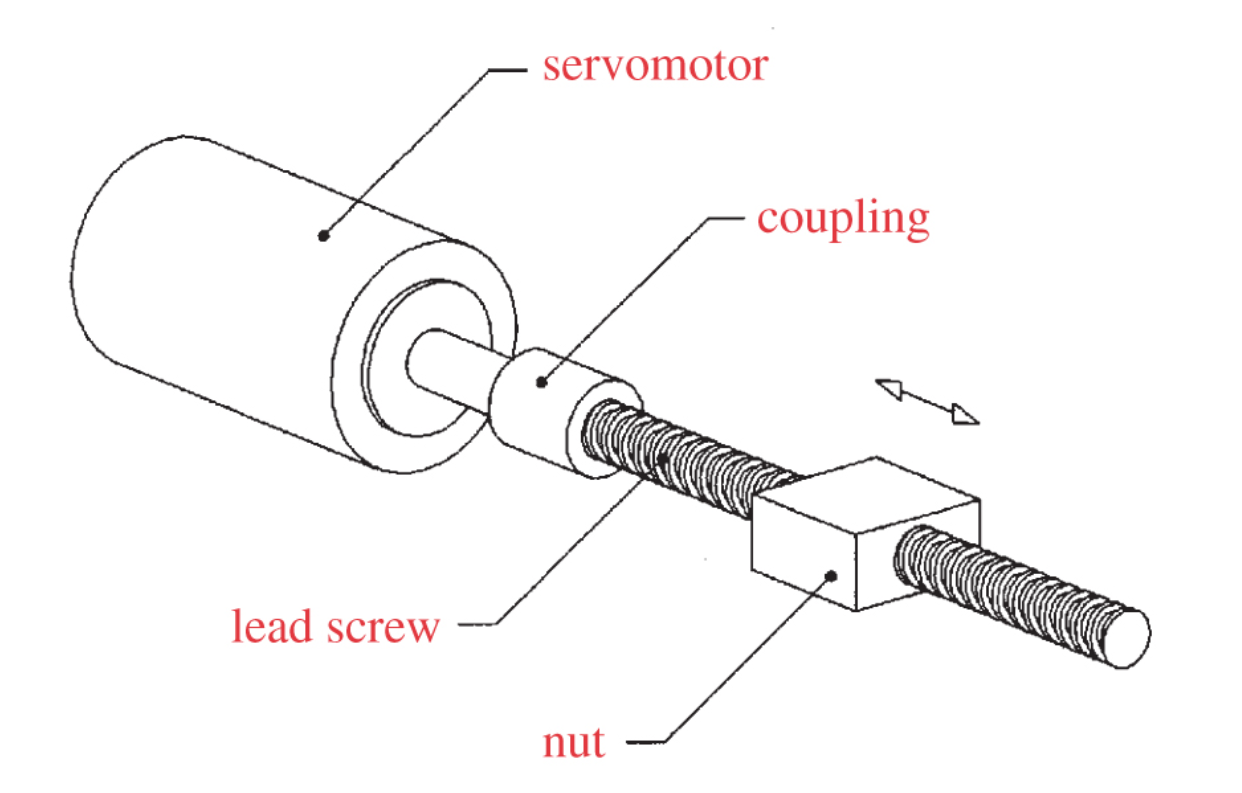
\includegraphics[scale=0.1]{images/figure_15_5.png}
		
		\end{multicols}

		\href{https://en.wikipedia.org/wiki/Bridgeport_(machine_tool_brand)\#/media/File:Sharp_3_Axis_Vertical_Mill_Full_View.jpg}{wikipedia: bridgeport}
	
	\end{frame}

	% Section I - Frame III
	\begin{frame}[label=sectionI] \small
		\frametitle{\sectiontitleI}	
		Linear Actuator - General Purpose Machine Component

		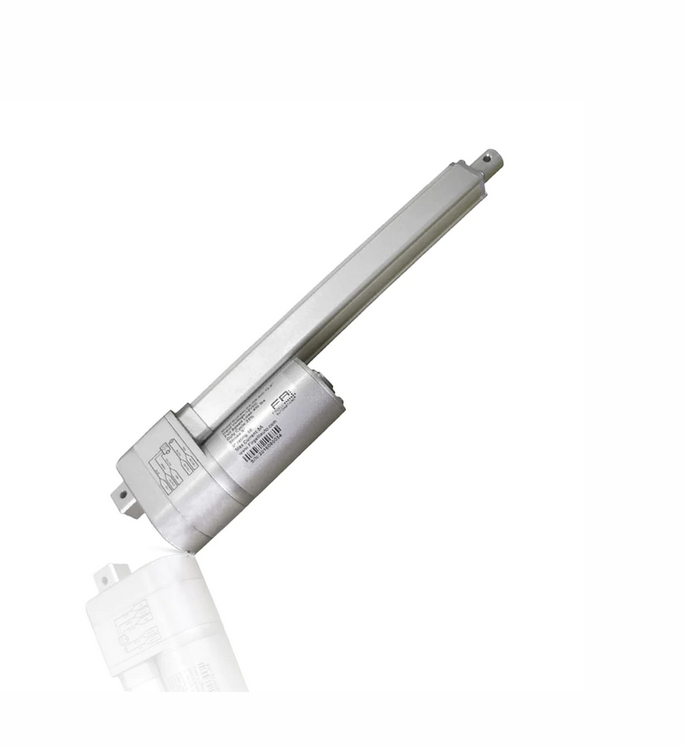
\includegraphics[scale=0.2]{images/fergelli_optical_feedback_actuator.png}

		\href{https://en.wikipedia.org/wiki/Linear_actuator\#/media/File:Linear_actuator_basic.gif}{wikipedia: animation}

	\end{frame}





	% Section I - Frame III
	\begin{frame}[label=sectionI] \small
		\frametitle{\sectiontitleI}	
		
		Advantages:
		\begin{itemize}
			\item large mechanical advantage possible
			\item capable of lifting or moving large loads 
			\item suitable for precision motion control
			\item self locking or back-drivable 
		\end{itemize}

		Disadvantages:
		\begin{itemize}
			\item Low Efficiency due to high friction
			\item High wear possible	
		\end{itemize}

	\end{frame}







% Section II
\section{\sectiontitleII}	

	% Section II - Frame I
	\begin{frame}[label=sectionII] \small
		\frametitle{\sectiontitleII}

		
		\begin{multicols}{2}
		The standard thread form is not strong enough for high load applications. Many power screw applications use a square, acme, or other type of thread for power transmission. \vspace{10mm}

		UN and ISO Standard Thread Form
		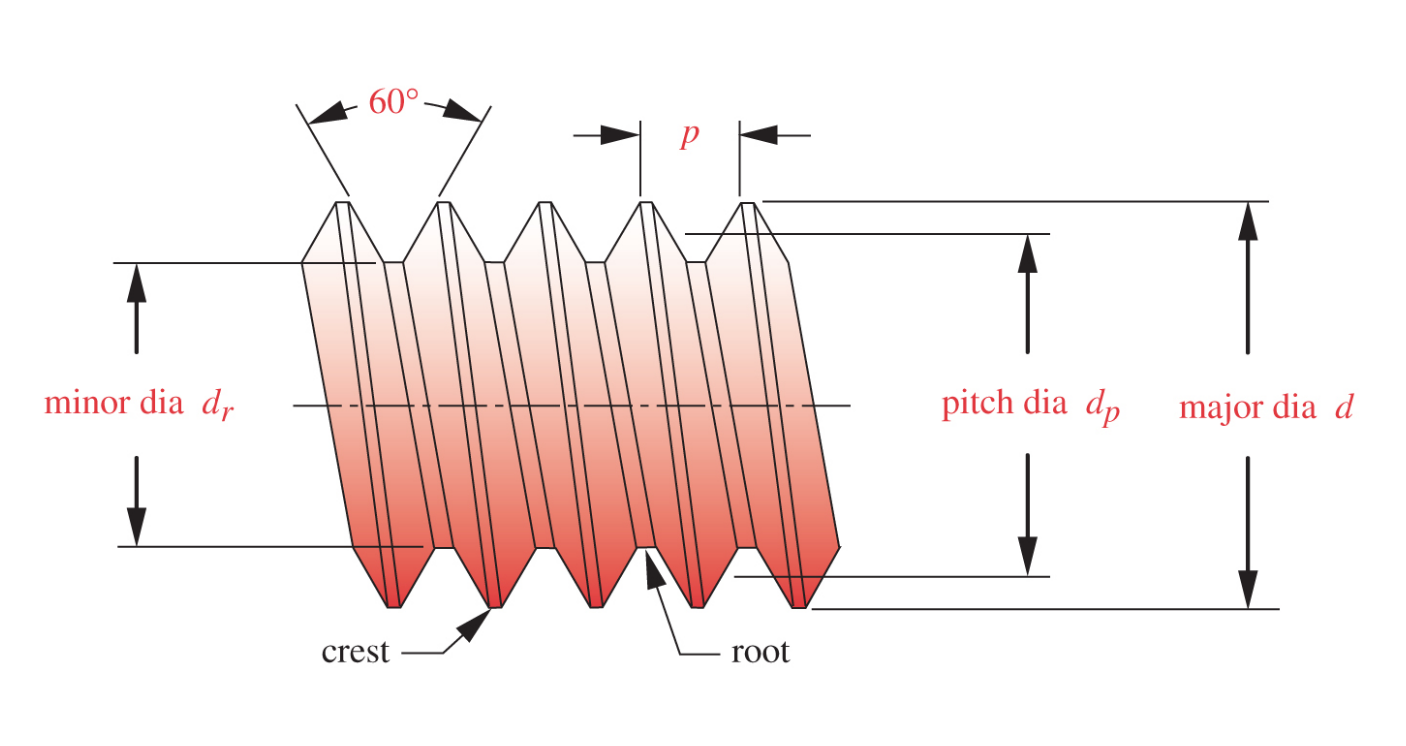
\includegraphics[scale=.1]{images/figure_15_2.png}
		\end{multicols}	

		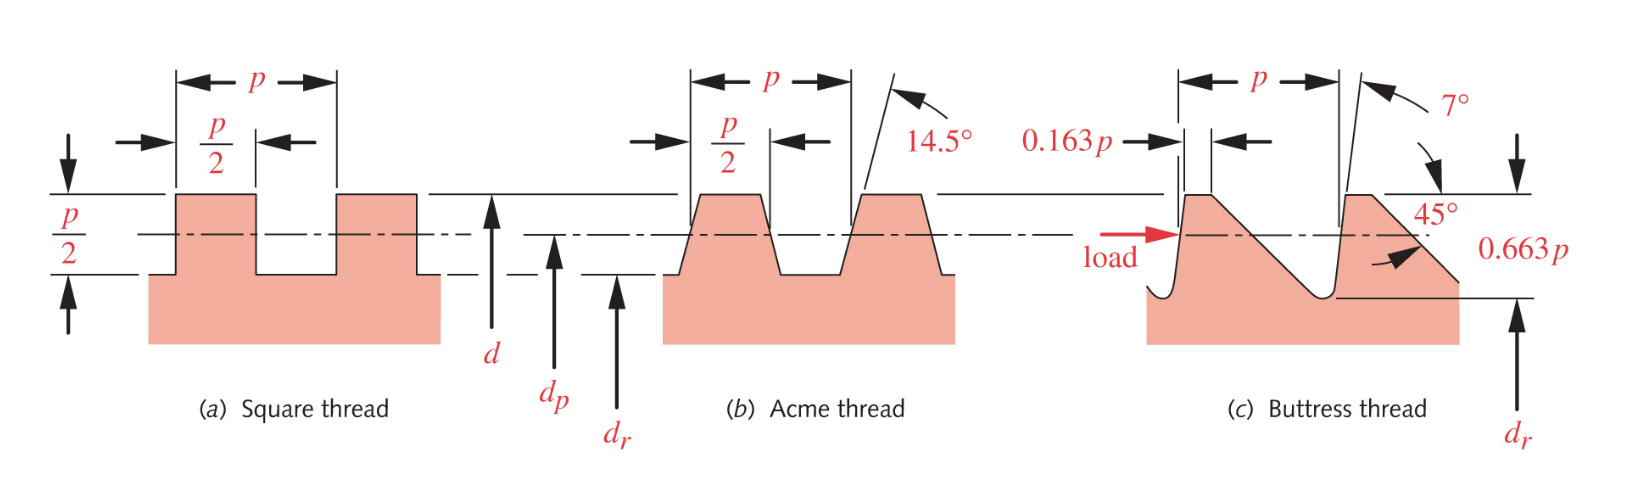
\includegraphics[scale=.15]{images/figure_15_3.png}	

	\end{frame}

	% Section II - Frame II
	\begin{frame}[label=sectionII] \small
		\frametitle{\sectiontitleII}


	\end{frame}

	% Section II - Frame III
	\begin{frame}[label=sectionII] \small
		\frametitle{\sectiontitleII}
		
	
	\end{frame}

	
% Section III
\section{\sectiontitleIII}	

	% Section III - Frame I
	\begin{frame}[label=sectionIII] \small
		\frametitle{\sectiontitleIII}
	 		

	
	        
	\end{frame}  

	% Section III - Frame I
	\begin{frame}[label=sectionIII] \small
		\frametitle{\sectiontitleIII}
	 		

		

	        
	\end{frame}  

	% Section III - Frame I
	\begin{frame}[label=sectionIII] \small
		\frametitle{\sectiontitleIII}
	 		

	

	\end{frame}  
	
	
% Section IV	
\section{\sectiontitleIV}	

	% Section IV - Frame I
    \begin{frame}[label=sectionIV] \small
		\frametitle{\sectiontitleIV}    

  		


	\end{frame}


% Section V	
\section{\sectiontitleV}	

	% Section V - Frame I
    \begin{frame}[label=sectionV] \small
	\frametitle{\sectiontitleV}    

  	

	\end{frame}

	% Section V - Frame II
    \begin{frame}[label=sectionV] \small
	\frametitle{\sectiontitleV}    

		

	\end{frame}
		
\end{document}